% Created 2021-12-22 Wed 20:44
% Intended LaTeX compiler: pdflatex
\documentclass[11pt]{article}
\usepackage[utf8]{inputenc}
\usepackage[T1]{fontenc}
\usepackage{graphicx}
\usepackage{longtable}
\usepackage{wrapfig}
\usepackage{rotating}
\usepackage[normalem]{ulem}
\usepackage{amsmath}
\usepackage{amssymb}
\usepackage{capt-of}
\usepackage{hyperref}
\usepackage{tikz-feynman}
\author{Alexander Neville}
\date{\today}
\title{Physics Notes}
\hypersetup{
 pdfauthor={Alexander Neville},
 pdftitle={Physics Notes},
 pdfkeywords={},
 pdfsubject={},
 pdfcreator={Emacs 27.2 (Org mode 9.6)}, 
 pdflang={English}}
\begin{document}

\maketitle
\tableofcontents


\section{Nuclear Physics}
\label{sec:org670e3eb}
\subsection{Radiation}
\label{sec:orgdcc366f}

Three types of radiation:

\begin{enumerate}
\item Alpha: \(^4_2\alpha\)
\item Beta: \(^{ \text{ } \text{ }0}_{-1}\beta^-\) / \(^{0}_{1}\beta^+\)
\item Gamma: \(\gamma\)
\end{enumerate}

\subsubsection{Alpha Emission}
\label{sec:orgdd05493}

An \(\alpha\) particle is composed of two neutrons and two protons. \(\alpha\) emission results in a different, smaller nuclide.

\[^A_ZX \rightarrow \text{} ^4_2\alpha + \text{} ^{A-4}_{Z-2}Y\]

\subsubsection{Beta Minus Decay}
\label{sec:orgcd3d911}

A \(\beta^-\) particle is an electron. During \(\beta^-\) emission, a neutron in a neutron-rich nucleus decays into a proton. The underlying change is the conversion of a \emph{down quark} into an \emph{up quark}.

\[^A_ZX \rightarrow \text{} ^{ \text{ } \text{ }0}_{-1}\beta + \text{} ^{\text{ } \text{ }A}_{Z+1}Y + \bar{\nu}_e\]


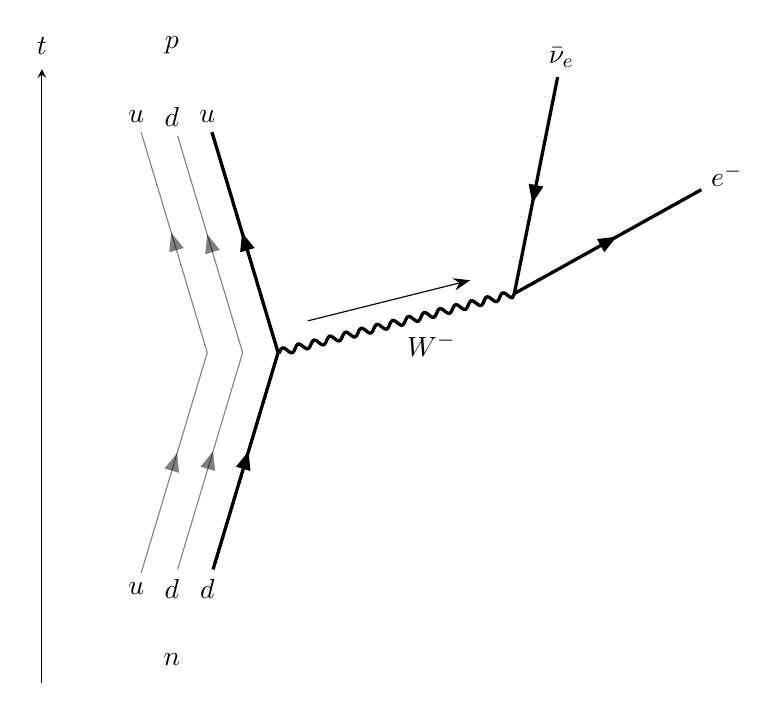
\begin{tikzpicture}[x=30mm, y=30mm]
\begin{feynman}
    \vertex (i1) {\(u\)};
    \vertex[right=.15 of i1] (i2) {\(d\)};
    \vertex[right=.15 of i2] (i3) {\(d\)};
    \vertex[below=.3 of i2] (n) {\(n\)};

    \vertex[above=2 of i1] (f1) {\(u\)};
    \vertex[right=.15 of f1] (f2) {\(d\)};
    \vertex[right=.15 of f2] (f3) {\(u\)};
    \vertex[above=.3 of f2] (p) {\(p\)};

    \vertex[above=1 of i3] (a);
    \vertex[right=.15 of a] (b);
    \vertex[right=.15 of b] (c);

    \vertex at ($(c) + (1,.25)$) (d);
    \vertex at ($(d) + (.2, 1)$) (f4) {\(\bar{\nu}_e\)};
    \vertex at ($(d) + (.9,.5)$) (f5) {\(e^-\)};
\diagram*{
    (i1) -- [fermion, opacity=0.5] (a) -- [fermion, opacity=0.5] (f1),
    (i2) -- [fermion, opacity=0.5] (b) -- [fermion, opacity=0.5] (f2),
    (i3) -- [fermion, very thick] (c) -- [fermion, very thick] (f3),
    (c) -- [boson, edge label'=\(W^-\), momentum, very thick] (d),
    (d) -- [fermion, very thick] (f5),
    (d) -- [anti fermion, very thick] (f4),
};

\draw[-stealth] (-.4,-.4) -- (-.4,2.2);
\node at (-.4,2.3) {\(t\)};
\end{feynman}
\end{tikzpicture}

\subsubsection{Beta Plus Decay}
\label{sec:org1361b5e}

A \(\beta^+\) particle is a positron. During \(\beta^+\) emission, a proton in a proton-rich nucleus decays into a neutron. The underlying change is the conversion of an \emph{up quark} into an \emph{down quark}.

\[^A_ZX \rightarrow \text{} ^{ \text{ } \text{ }0}_{+1}\beta + \text{} ^{\text{ } \text{ }A}_{Z-1}Y + \nu_e\]


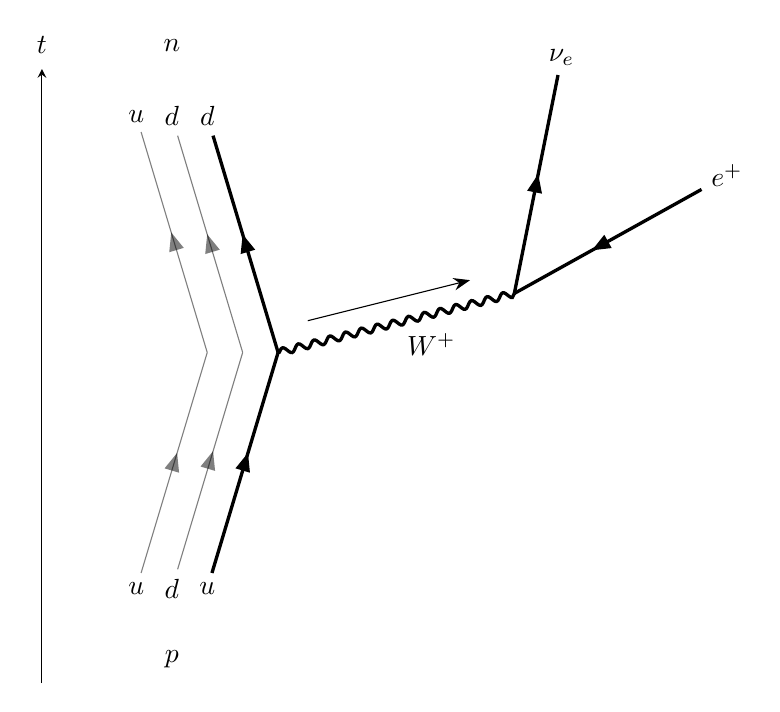
\begin{tikzpicture}[x=30mm, y=30mm]
\begin{feynman}
    \vertex (i1) {\(u\)};
    \vertex[right=.15 of i1] (i2) {\(d\)};
    \vertex[right=.15 of i2] (i3) {\(u\)};
    \vertex[below=.3 of i2] (n) {\(p\)};

    \vertex[above=2 of i1] (f1) {\(u\)};
    \vertex[right=.15 of f1] (f2) {\(d\)};
    \vertex[right=.15 of f2] (f3) {\(d\)};
    \vertex[above=.3 of f2] (p) {\(n\)};

    \vertex[above=1 of i3] (a);
    \vertex[right=.15 of a] (b);
    \vertex[right=.15 of b] (c);

    \vertex at ($(c) + (1,.25)$) (d);
    \vertex at ($(d) + (.2, 1)$) (f4) {\(\nu_e\)};
    \vertex at ($(d) + (.9,.5)$) (f5) {\(e^+\)};
\diagram*{
    (i1) -- [fermion, opacity=0.5] (a) -- [fermion, opacity=0.5] (f1),
    (i2) -- [fermion, opacity=0.5] (b) -- [fermion, opacity=0.5] (f2),
    (i3) -- [fermion, very thick] (c) -- [fermion, very thick] (f3),
    (c) -- [boson, edge label'=\(W^+\), momentum, very thick] (d),
    (d) -- [anti fermion, very thick] (f5),
    (d) -- [fermion, very thick] (f4),
};

\draw[-stealth] (-.4,-.4) -- (-.4,2.2);
\node at (-.4,2.3) {\(t\)};
\end{feynman}
\end{tikzpicture}

\subsubsection{Electron Capture}
\label{sec:org5fbe859}

A proton-rich nucleus could also undergo \emph{electron capture}. In this type of decay a proton changes into a neutron after capturing an inner shell electron.

\[^A_ZX + ^{ \text{ } \text{ }0}_{-1}\beta \rightarrow \text{} ^{\text{ } \text{ }A}_{Z-1}Y + \nu_e\]


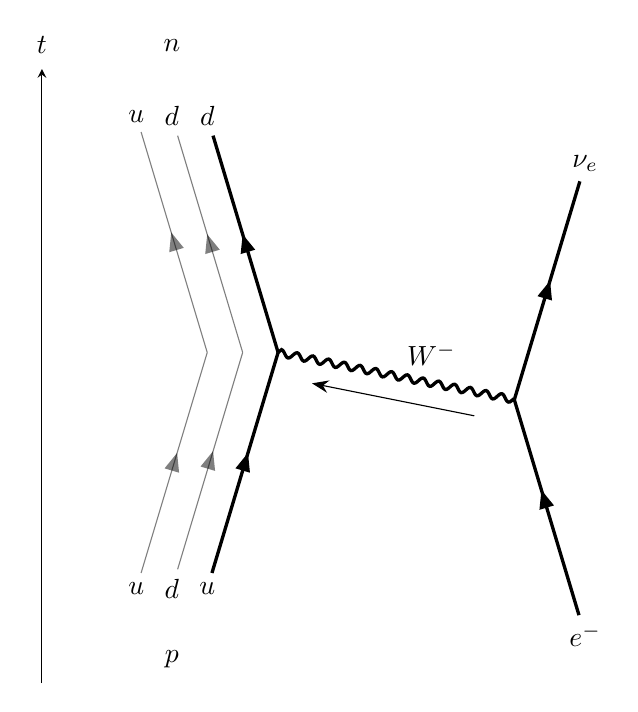
\begin{tikzpicture}[x=30mm, y=30mm]
\begin{feynman}
    \vertex (i1) {\(u\)};
    \vertex[right=.15 of i1] (i2) {\(d\)};
    \vertex[right=.15 of i2] (i3) {\(u\)};
    \vertex[below=.3 of i2] (n) {\(p\)};

    \vertex[above=2 of i1] (f1) {\(u\)};
    \vertex[right=.15 of f1] (f2) {\(d\)};
    \vertex[right=.15 of f2] (f3) {\(d\)};
    \vertex[above=.3 of f2] (p) {\(n\)};

    \vertex[above=1 of i3] (a);
    \vertex[right=.15 of a] (b);
    \vertex[right=.15 of b] (c);

    \vertex at ($(c) + (1,-.2)$) (d);
    \vertex at ($(d) + (.3, 1)$) (f4) {\(\nu_e\)};
    \vertex at ($(d) + (.3,-1)$) (f5) {\(e^-\)};
\diagram*{
    (i1) -- [fermion, opacity=0.5] (a) -- [fermion, opacity=0.5] (f1),
    (i2) -- [fermion, opacity=0.5] (b) -- [fermion, opacity=0.5] (f2),
    (i3) -- [fermion, very thick] (c) -- [fermion, very thick] (f3),
    (d) -- [boson, edge label'=\(W^-\), momentum, very thick] (c),
    (d) -- [anti fermion, very thick] (f5),
    (d) -- [fermion, very thick] (f4),
};

\draw[-stealth] (-.4,-.4) -- (-.4,2.2);
\node at (-.4,2.3) {\(t\)};
\end{feynman}
\end{tikzpicture}

The nature of the \emph{W boson} is not significant/distinguishable. The same diagram could be written:


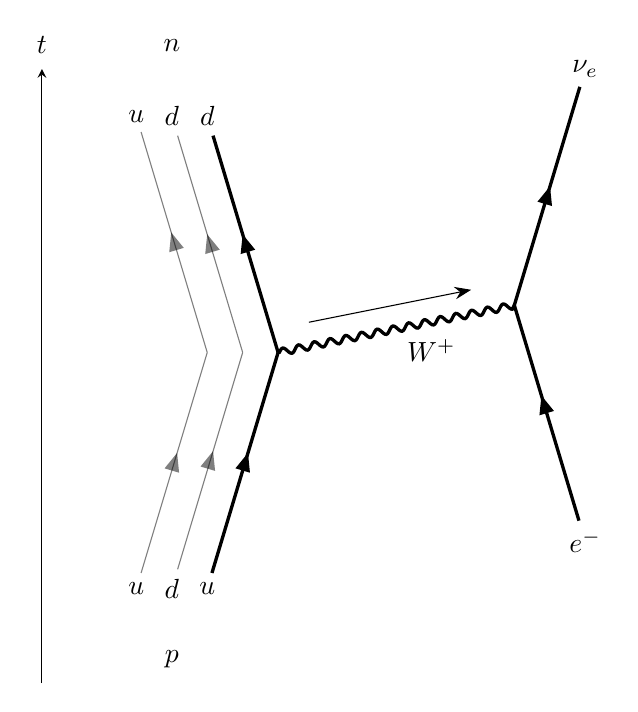
\begin{tikzpicture}[x=30mm, y=30mm]
\begin{feynman}
    \vertex (i1) {\(u\)};
    \vertex[right=.15 of i1] (i2) {\(d\)};
    \vertex[right=.15 of i2] (i3) {\(u\)};
    \vertex[below=.3 of i2] (n) {\(p\)};

    \vertex[above=2 of i1] (f1) {\(u\)};
    \vertex[right=.15 of f1] (f2) {\(d\)};
    \vertex[right=.15 of f2] (f3) {\(d\)};
    \vertex[above=.3 of f2] (p) {\(n\)};

    \vertex[above=1 of i3] (a);
    \vertex[right=.15 of a] (b);
    \vertex[right=.15 of b] (c);

    \vertex at ($(c) + (1,.2)$) (d);
    \vertex at ($(d) + (.3, 1)$) (f4) {\(\nu_e\)};
    \vertex at ($(d) + (.3,-1)$) (f5) {\(e^-\)};
\diagram*{
    (i1) -- [fermion, opacity=0.5] (a) -- [fermion, opacity=0.5] (f1),
    (i2) -- [fermion, opacity=0.5] (b) -- [fermion, opacity=0.5] (f2),
    (i3) -- [fermion, very thick] (c) -- [fermion, very thick] (f3),
    (c) -- [boson, edge label'=\(W^+\), momentum, very thick] (d),
    (d) -- [anti fermion, very thick] (f5),
    (d) -- [fermion, very thick] (f4),
};

\draw[-stealth] (-.4,-.4) -- (-.4,2.2);
\node at (-.4,2.3) {\(t\)};
\end{feynman}
\end{tikzpicture}

\subsubsection{Gamma Emission}
\label{sec:org6663cc3}

There is no change to the number of nucleons in the nucleus when a \(\gamma\) photon is emitted. This type of emission usually happens if the nucleus is in an excited state after one of the previous types of emission.

\subsection{Inverse Square Law}
\label{sec:orge065466}

The intensity \(I\) of \(\gamma\) radiation is the energy transferred per second per unit area. Assuming a point source emits \(n\) \(\gamma\) photons per second and each photon has the energy \(hf\), the total energy emitted by the source per second is \(nhf\). These photons are free to leave the source in any direction, so at distance \(r\) from the source all the photons will pass through an area equal to the \emph{S.A.} of a sphere with radius \(r\). This equation represents the intensity of radiation from a point source at distance \(r\):

\[I = \dfrac{nhf}{4 \pi r^2}\]

\subsection{Hazards of Radiation}
\label{sec:orgde935c0}

Ionising radiation is damaging to living cells. It may cause cells to die, mutate or grow uncontrollably. The consequences may be felt by the affected individual, which is described as \emph{somatic effects}, or passed onto future generations \emph{genetically}.

To best mitigate the risks of radiation, sources should be kept in \emph{lead-lined} containers to reduce any \(\gamma\) emission from the source to background level. These sources may be kept in a secure, locked-away location and exposure / use of the source should be recorded.

During use, solid sources should be handled with handling tools, to keep the source at a distance from the body. This reduces the intensity of \(\gamma\) radiation incident on the handler and would ideally put their body beyond the range of \(\alpha\) or \(\beta\) particles. Liquid, gaseous and powdered sources should be kept in sealed containers, so they are not accidentally inhaled, ingested or split.

\subsection{Radioactive Decay}
\label{sec:orge697889}

If a radioactive isotope of element \(X\) undergoes \(\alpha\) or \(\beta\) emission, it is no longer a nucleus of the same element, due to the change in proton number. If this nucleus was one of many in a sample of a particular isotope, the number of nuclei of this isotope will decrease as individual nuclei decay. The same relationship is true of the mass of the original isotope; the mass will decrease as nuclei decay. There are three important quantities surrounding radioactive decay:

\begin{itemize}
\item The \emph{half-life} \(T_{1/2}\) of a radioactive isotope is the time take for the mass (or any other specific property) to decrease to half the initial value.

\item The \emph{activity} \(A\) of a radioactive isotope is the number of nuclei disintegrating per second, corresponds to the rate of changes of nuclei of the initial isotope. The unit of activity is the \emph{Becquerel} (Bq), where 1Bq is one disintegration per second.

\item The \emph{decay constant} \(\lambda\) is the probability of an individual nucleus decaying per unit time (usually one second).
\end{itemize}

The decay of a single nucleus is impossible to predict. Every nucleus of an isotope in a sample has an equal probability of decaying in a given interval. For a large sample of a radioactive isotope \(X\), the number of nuclei which disintegrate \(\Delta N\) in a given time period \(\Delta t\) is related to the initial number of nuclei \(N_0\), via the decay constant.

\subsubsection{Decay Constant}
\label{sec:orga01f62e}

The probability of a single decay is the fraction of the initial number of nuclei of \(X\) which decay per second. This is called the \emph{decay constant}, and is represented with the symbol \(\lambda\). If reference is made to \emph{decay} or its decreasing nature, there is no need to include a minus sign.

\[\lambda = \dfrac{\Delta N}{N_0}/\Delta t\]

The change in number of nuclei for a combination of the given factors can be obtained by rearranging the equation above. Note the presence of the minus sign here indicating decrease.

\[ \Delta N = - \lambda N_0 \Delta t\]

\subsubsection{Activity}
\label{sec:org6c83f32}

The activity of the isotope is the number of nuclei which disintegrate per second and it is proportional to the value of \(N_0\). An expression for \(A\) can be obtained as follows:

\[ \dfrac{\Delta N}{\Delta t} = - \lambda N_0\]

\[ A = - \lambda N_0\]

Therefore the activity of \(N\) nuclei of a particular isotope can also be written simply:

\[ A = \lambda N\]

\subsubsection{Decay Curves}
\label{sec:org8719a67}

As the activity, or rate of change of nuclei of \(X\), is proportional to the current number of nuclei \(N\) of \(X\), the relationship between \(t\) and \(N\) is one of exponential decay. The number of nuclei remaining after a particular time period is proportional to \(N_0\).

\[N = N_0 e^{- \lambda t}\]

\begin{center}
\includegraphics[width=.9\linewidth]{./images/c-14_decay.png}
\end{center}

Both activity and mass are directly related to the number of nuclei.

\[m = m_0 e^{- \lambda t}\]
\[A = A_0 e^{- \lambda t}\]

\subsubsection{Half-life}
\label{sec:org2e59fce}

Half-life can be linked to the decay constant. When \(t= T_{1/2}\), the number of nuclei remaining is \(N = 0.5N_0\). With these equations, substitutions can be made:

\(0.5N_0 = N_0 e^{-\lambda T_{1/2}}\)

\(0.5 = e^{-\lambda T_{1/2}}\)

\(\ln (0.5) = -\lambda T_{1/2}\)

\(-\ln (0.5) = \lambda T_{1/2}\)

\(\ln (0.5^{-1}) = \lambda T_{1/2}\)

\(\ln (2) = \lambda T_{1/2}\)

\(T_{1/2} = \dfrac{\ln(2)}{\lambda}\)

\begin{center}
\includegraphics[width=.9\linewidth]{./images/c-14_t_half.png}
\end{center}

\subsubsection{Nuclear Radius}
\label{sec:org74a3d2e}

The radius of a nucleus is proportional to the cube root of the nucleon number and the constant \(r_0\), which is equal to 1.05fm.

\[R = r_0 A^{1/3}\]

\(V = \dfrac{4}{3} \pi R^3 = \dfrac{4}{3} \pi (r_0 A^{1/3})^3 = \dfrac{4}{3} \pi {r_0}^3 A\)

Seeing as the mass of a nucleus is equal to \(Au\), where \(u\) is the atomic mass unit, the density of any nucleus is constant.

\(\rho = \dfrac{Au}{4/3 \text{ } \pi {r_0}^3 A} = \dfrac{1u}{4/3 \text{ } \pi {r_0}^3}\)

When evaluated, the density of a nucleus of any element is \(3.4 \times 10^{17}\).
\end{document}
